\section{Evklidske in origami konstrukcije}
\label{pogl:aksiomi}

Kraj in čas izvora origamija nista jasno določena. Nekateri viri zatrjujejo, da izhaja iz Japonske, drugi ga pripisujejo Kitajski, tretji se ne strinjajo z nobeno od teh dveh možnosti. Verjetno so umetnost zlaganja odkrili še pred izumom papirja, za katerega je l. 105 po Kr. poskrbel kitajski dvorni uradnik Cai Lun, saj se da npr.\ zlagati tudi robce iz blaga~\cite{robinson2024}. Je pa papir idealen material za zlaganje. Japonska beseda \emph{origami} kot umetnost zgibanja papirja (``oru'' -- prepogibati, ``kami'' -- papir) se je na Daljnem vzhodu začela uporabljati proti koncu 19. stoletja.

Povečano zanimanje za origami v matematiki se je začelo v 2.\ pol.\ 20.\ stoletja in s seboj prineslo množično izhajanje literature o povezavi origamija z matematiko, fiziko, astronomijo, računalništvom, kemijo in še mnogimi drugimi vedami~\cite{zore2022}. V angleščini je tako za matematično raziskovanje s prepogibanjem papirja nastalo poimenovanje ``\emph{origamics}''. V slovenščini uradnega prevoda še ni, Grahor pa v~\cite[str.\ 5]{sgv2016} po zgledu poimenovanj veliko znanstvenih disciplin (\emph{mathematics} -- matematika, \emph{physics} -- fizika itd.) predlaga termin ``origamika''.

\subsection{Evklidovi postulati in evklidske konstrukcije}

Preden si pogledamo, kaj lahko s prepogibanjem papirja konstruiramo, se spomnimo, na čem temelji evklidska geometrija. Za njenega očeta štejemo grškega matematika Evklida\footnote{O življenju tega aleksandrijskega učenjaka ne vemo nič gotovega, je pa zelo verjetno živel za časa prvega Ptolemaja (faraon v času 306--283 pr.\ Kr.)~\cite[str.\ 61]{struik1986}.}, ki je napisal zelo znano zbirko trinajstih knjig pod skupnim imenom \emph{Elementi}. V njih obravnavana snov temelji na strogo logični izpeljavi izrekov iz definicij\footnote{\emph{Definicija} je nedvoumno jasna opredelitev novega pojma.}, aksiomov\footnote{\emph{Aksiom} je temeljna resnica ali načelo, ki ne potrebuje dokazov (oz.\ dokaz sploh ne obstaja) in vedno velja.} in postulatov\footnote{\emph{Postulat} je predpostavka oz.\ zahteva. Evklid med aksiomi in postulati ni postavil jasne razlike, Aristotel pa je postulat od aksioma ločil po tem, da gre pri prvem bolj za hipotezo kot temeljno resnico, vendar se njene veljavnosti ne dokazuje, temveč privzame kot veljavno~\cite[str.\ 122]{euclidI}. V primeru petega Evklidovega postulata se bomo spomnili, da nam to, ali ga privzamemo ali ne, poda različne geometrije. Danes med pojmoma ne ločujemo~\cite[str.\ 2]{geometricconstructions}.}. Še danes večina osnovno- in srednješolske geometrije izvira prav iz prvih šestih knjig Elementov.

Prva knjiga nas še posebej zanima. V njej je Evklid najprej definiral osnovne pojme -- točka, premica, površina, ravnina, ravninski kot, pravi kot, ostri kot, topi kot, krog, središče kroga, premer, enakostranični in enakokraki trikotnik, kvadrat \ldots ter nazadnje upeljal še pojem vzporednih premic~\cite{euclidI}. Nato je zapisal znamenitih pet postulatov, iz katerih izhaja vsa evklidska geometrija:

\renewcommand{\thepostulat}{P\arabic{postulat}}

\begin{postulat}
    \label{post:P1}
    Med dvema poljubnima točkama je mogoče narisati ravno črto.
\end{postulat}
\begin{postulat}
    \label{post:P2}
    Vsako ravno črto je mogoče na obeh koncih podaljšati.
\end{postulat}
\begin{postulat}
    \label{post:P3}
    Mogoče je narisati krožnico s poljubnim središčem in poljubnim polmerom.
\end{postulat}
\begin{postulat}
    \label{post:P4}
    Vsi pravi koti so med seboj skladni.
\end{postulat}
\begin{postulat}
    \label{post:P5}
    Če poljubni ravni črti sekamo s tretjo ravno črto (prečnico) in je vsota notranjih kotov eni strani prečnice manjša od dveh pravih kotov, potem se dani premici, če ju dovolj podaljšamo, sekata na tej strani prečnice.
    \opomba{Vemo že, da je postulat~\ref{post:P5} ekvivalenten \emph{aksiomu o vzporednicah}, ki pravi, da skozi dano točko, ki ne leži na dani premici, poteka natanko ena vzporednica k tej premici.}
\end{postulat}

\begin{definicija}
    \emph{Evklidske konstrukcije} so konstrukcije točk, daljic, premic, krožnic in tistih geometrijskih objektov, ki jih je mogoče konstruirati le z uporabo t.\ i.\ \emph{evklidskih orodij}:
    \begin{itemize}
        \item neoznačeno in neskončno dolgo ravnilo (angl.\ \emph{straightedge}) in
        \item šestilo, ki ne prenaša razdalj (ko ga dvignemo od podlage, se njegova kraka zložita skupaj).
    \end{itemize}
\end{definicija}

\begin{opomba}
    \label{opom:solsko_sestilo}
    Da se pokazati, da lahko za konstrukcije ekvivalentno uporabimo tudi šestilo, ki prenaša razdalje~\cite[str.\ 6--7]{geometricconstructions}. Zato imamo odslej z izrazom \emph{šestilo} v mislih kar moderno šolsko šestilo.
\end{opomba}

Konstrukcije iz definicije temeljijo na postulatih~\ref{post:P1}--\ref{post:P3}. Vendar je to dovolj, da lahko le z neoznačenim ravnilom in šestilom konstruiramo premice, kote, simetrale kotov in daljic, krožnice, nekatere geometrijske like in še kaj.

Izkaže pa se, da z evklidskim orodjem ne moremo konstruirati česarkoli -- kot zelo znane primere lahko tu naštejemo tri starogrške probleme. Pri  \emph{kvadraturi kroga} nam evklidsko orodje ne zmore konstruirati razdalje $\sqrt{\pi}$, pri \emph{podvojitvi kocke} razdalje $\sqrt{2}$, pri \emph{trisekciji kota} ne zmore poljubnega kota razdeliti na tri enake dele. Drugi in tretji problem sta, verjetno za marsikoga presenetljivo, rešljiva z origamijem. V razdelku~\ref{podpogl:starogrskiproblemi} si bomo pogledali njuni rešitvi, sedaj pa podrobneje spoznajmo še konstrukcije, ki jih dobimo s prepogibanjem papirja.

\subsection{Origami konstrukcije}
\label{origami_konstrukcije}

V nalogi se bomo omejili le na prepogibanje v ravnini in se z trodimenzionalni modeli ne ukvarjamo. Bralec je ob branju povabljen, da opisane konstrukcije praktično preizkusi tudi sam. Pri izbiri papirja je priporočljiv rahlo prosojen papir, skozi katerega se vidijo morebitne označbe točk in premic s svinčnikom (npr.\ navaden kuhinjski papir za peko).

Bistvo origamija je, da prepogibamo list papirja, ki nam služi kot model evklidske ravnine, vendar si moramo določiti nekaj pravil:
\begin{itemize}
    \item konstruiramo le \emph{ravne} pregibe,
    \item pregibe opravljamo \emph{po enega naenkrat}, torej po vsakem pregibu papir nazaj razgrnemo,
    \item ne uporabljamo drugih orodij, kot so škarje, lepilo ipd.,
    \item pomožne točke, za katere vemo, da jih znamo konstruirati, ampak bi nam pomožni pregibi zmanjšali preglednost konstrukcije, lahko označimo s pisalom (npr.\ zrcaljene točke v nadaljevanju). Prav tako lahko že konstruirane točke in premice s pisalom in s pomočjo ravnila močneje poudarimo.
\end{itemize}
Ker so pregibi ravni, nam služijo kot modeli premic, modeli točk pa so njihova presečišča. Dogovorimo se še, da ne opravljamo naključnih pregibov, temveč papir prepogibamo tako, da se objekti na njem (točke in premice) prekrijejo. Zato moramo na začetku imeti na listu že nekaj danih objektov (npr.\ dve različni točki ali premico in točko, ki ne leži na njej). Če poskusimo razmisliti, kaj so potem vsi možni dovoljeni prepogibi, pridemo do sledečih petih možnosti (za njihov slikovni prikaz gl.\ \cite[str.\ 25--26]{hull2020}):
\begin{itemize}
    \item točko prepognemo na drugo točko (en možen pregib),
    \item točko prepognemo samo vase (neskončno možnih pregibov),
    \item točko prepognemo na premico (neskončno možnih pregibov),
    \item premico prepognemo na drugo premico (en ali dva možna pregiba) in
    \item premico prepognemo samo vase (neskončno možnih pregibov).
\end{itemize}

\begin{definicija}
    \label{def:origami_konstruktibilnost}
    \emph{Origami konstrukcije} so konstrukcije točk, premic in tistih geometrijskih objektov, ki jih je mogoče konstruirati le z ravnimi in enkratnimi prepogibi iz zgornjega seznama.
\end{definicija}

\subsubsection{Origami operacije}
\label{podpodpogl:operacije}

V zadnjem stoletju se je preko več matematikov (Jacques Justin, Peter Messer, Benedetto Scimemi, Humiaki Huzita, Koshiro Hatori, George E.\ Martin idr.; nekateri so med seboj sodelovali, drugi so delovali neodvisno) skozi čas izoblikoval seznam t.\ i.\ \emph{origami operacij}\footnote{Najbolj znanih pod imenom \emph{Huzita-Hatori aksiomi}, vendar izraz \emph{aksiom} tu ni primeren, saj bomo kmalu pokazali, da se med seboj prepletajo so nekateri izmed njih kombinacija drugih. Prav tako v nalogi opustimo ime avtorjev, ker je seznam delo veliko več matematikov kot le Hatorije in Huzite.}, ki zajamejo vseh pet možnosti prepogibanja. Da so to zadostne operacije za katerokoli origami konstrukcijo, si bomo pogledali v razdelku~\ref{podpogl:zadost_potr_op}.

Seznam se je med avtorji razlikoval v številu (gl.\ ~\cite[str.\ 29--30]{hull2020}), kot končen seznam pa bomo tu navedli vseh osem naštetih -- na prvi pogled različnih -- operacij. Najprej jih naštejmo, potem pa si ob sledečih slikah poglejmo še prikaz opisanih konstrukcij. Videli bomo, da moramo pri nekaterih operacijah ločiti več primerov~\cite{michael2005, zore2022}.

\renewcommand{\theoperacija}{O\arabic{operacija}}

\begin{operacija}
    \label{op:O1}
    Za poljubni točki $A$ in $B$ obstaja natanko en pregib $p$, ki gre skoznju.
\end{operacija}
\begin{operacija}
    \label{op:O2}
    Za poljubni premici lahko določimo njuno presečišče, če obstaja.
\end{operacija}
\begin{operacija}
    \label{op:O3}
    Za poljubni točki $A$ in $B$ obstaja natanko en pregib $p$, da se točki pokrijeta.
\end{operacija}
\begin{operacija}
    \label{op:O4}
    Za poljubni premici $a$ in $b$ obstaja pregib $p$, ki ju položi eno na drugo.
\end{operacija}
\begin{operacija}
    \label{op:O5}
    Za poljubno točko $A$ in premico $a$ obstaja natanko en pregib $p$ skozi točko $A$, ki je pravokoten na premico $a$.
\end{operacija}
\begin{operacija}
    \label{op:O6}
    Za primerno izbrani točki $A$ in $B$ ter premico $a$ obstaja pregib $p$ skozi točko $B$, ki točko $A$ položi na premico $a$.
\end{operacija}
\begin{operacija}
    \label{op:O7}
    Za primerno izbrani točki $A$ in $B$ ter premici $a$ in $b$ obstaja pregib $p$, ki točko $A$ položi na premico $a$ in točko $B$ na premico $b$.
\end{operacija}
\begin{operacija}
    \label{op:O8}
    Za poljubno točko $A$ ter nevzporedni premici $a$ in $b$ obstaja pregib $p$, ki je pravokoten na premico $b$ in točko $A$ položi na premico $a$.
\end{operacija}

Sedaj za vsako operacijo posebej poglejmo njeno konstrukcijo. Takoj opazimo, da je operacija~\ref{op:O1} ekvivalentna postulatu~\ref{post:P1}, kar nam lahko vzbudi zanimanje za povezavo med evklidskimi in origami konstrukcijami. Operacija~\ref{op:O2} je izvedljiva v vsakem primeru nevzporednih pregibov in nam omogoča določitev novih točk v našem modelu ravnine. Operacija~\ref{op:O3} pa nam poda konstrukcijo simetrale daljice $AB$ (slika~\ref{fig:O1-O3}) -- ko opravimo pregib in pustimo papir še zapognjen, je očitno, da so točke na pregibu enako oddaljene od točk $A$ in $B$.

\begin{figure}[h]
    \centering
    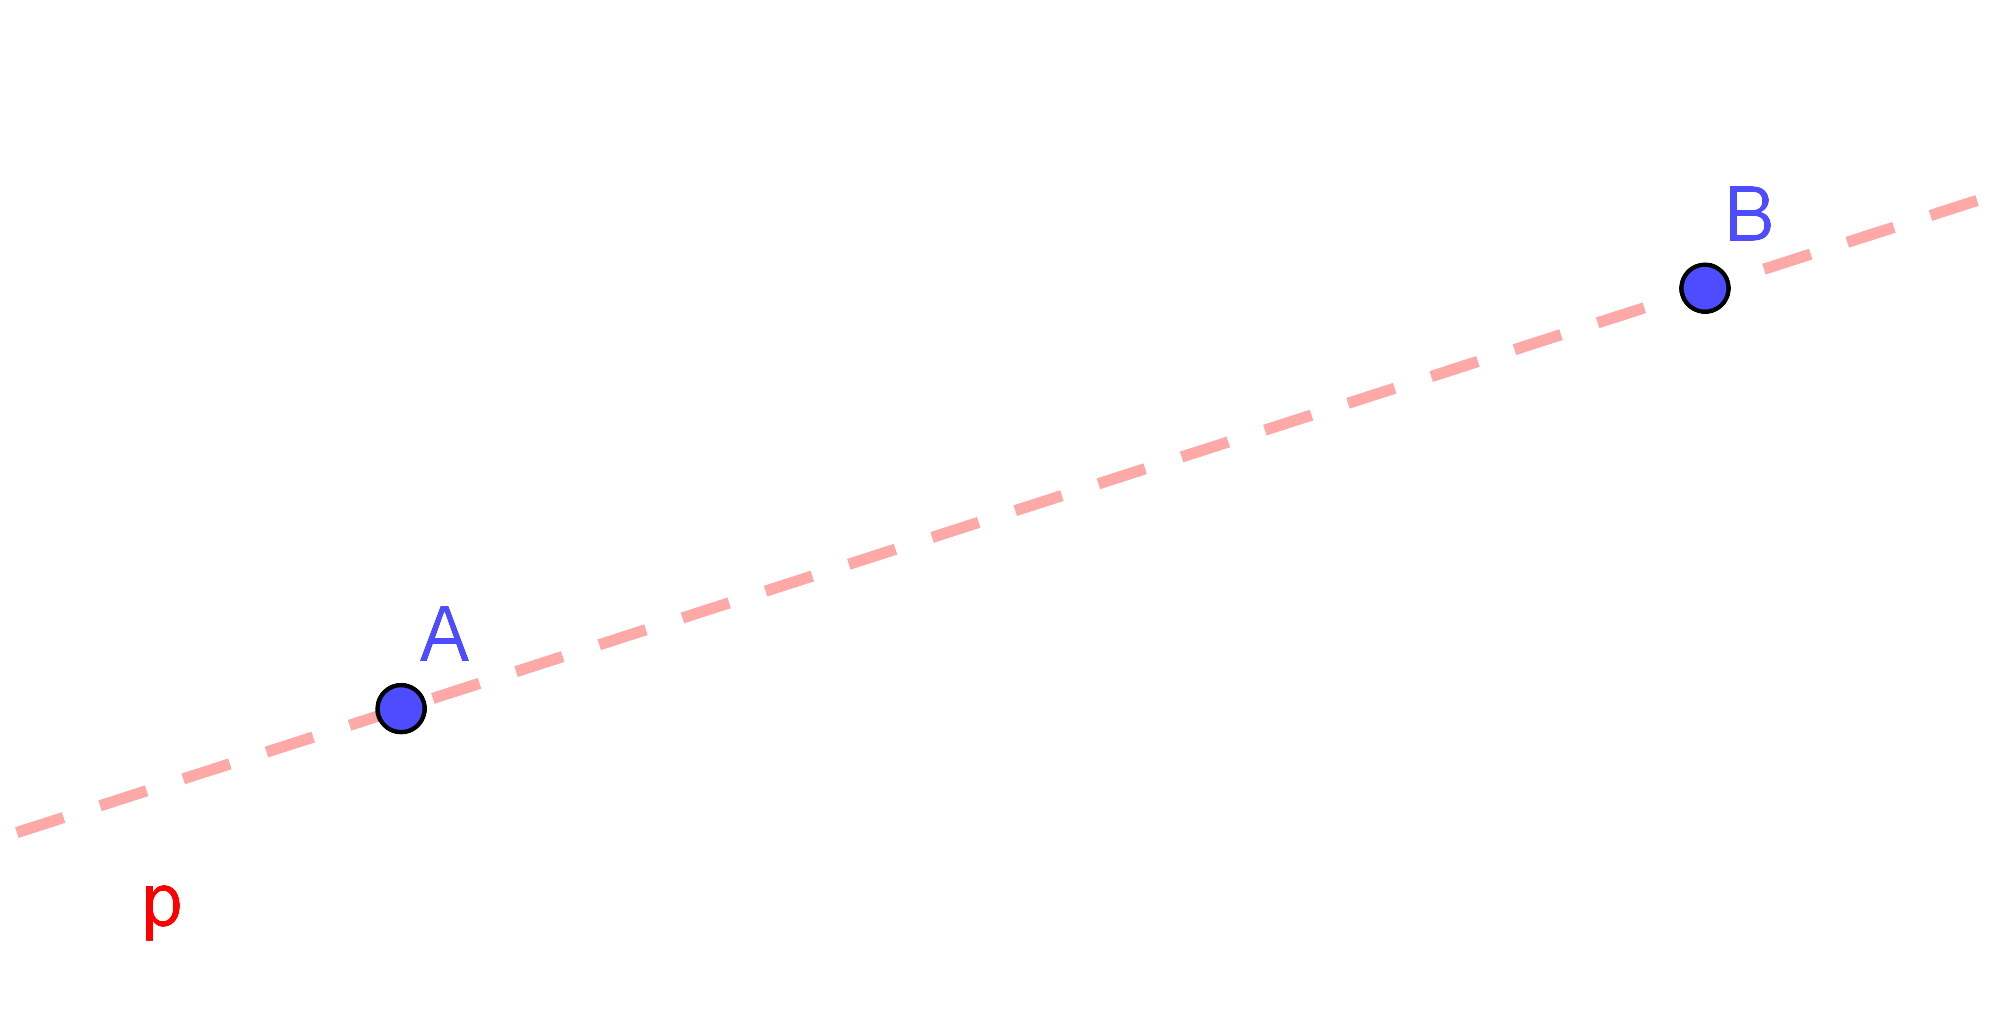
\includegraphics[width=0.4\textwidth]{images/origami_operacije/O1.png}
    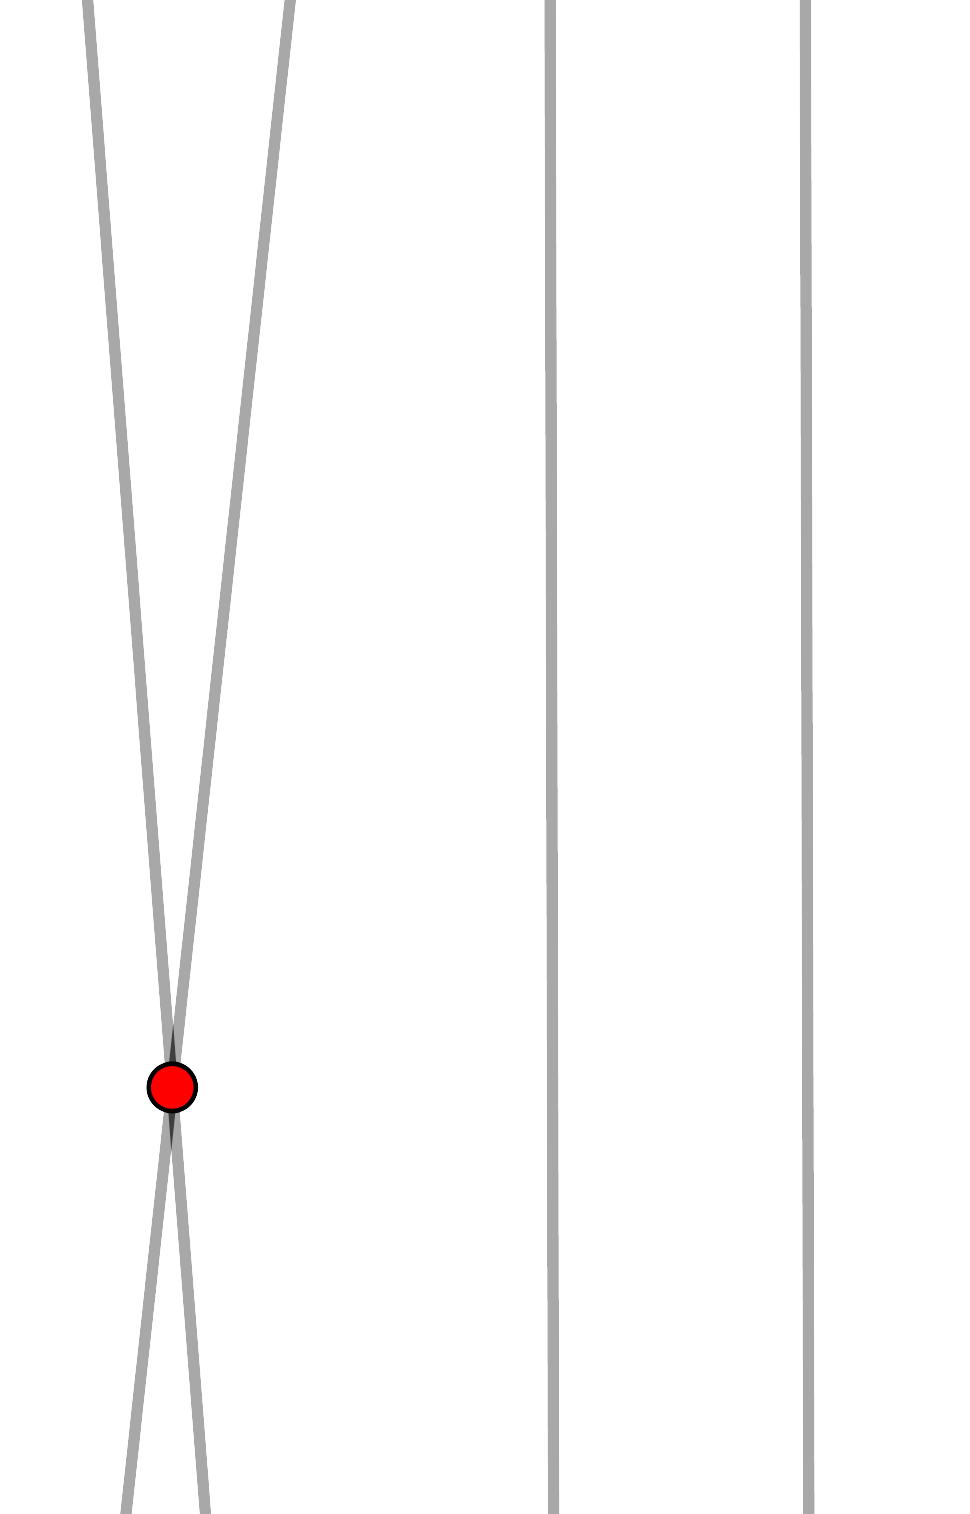
\includegraphics[width=0.2\textwidth]{images/origami_operacije/O2.png}
    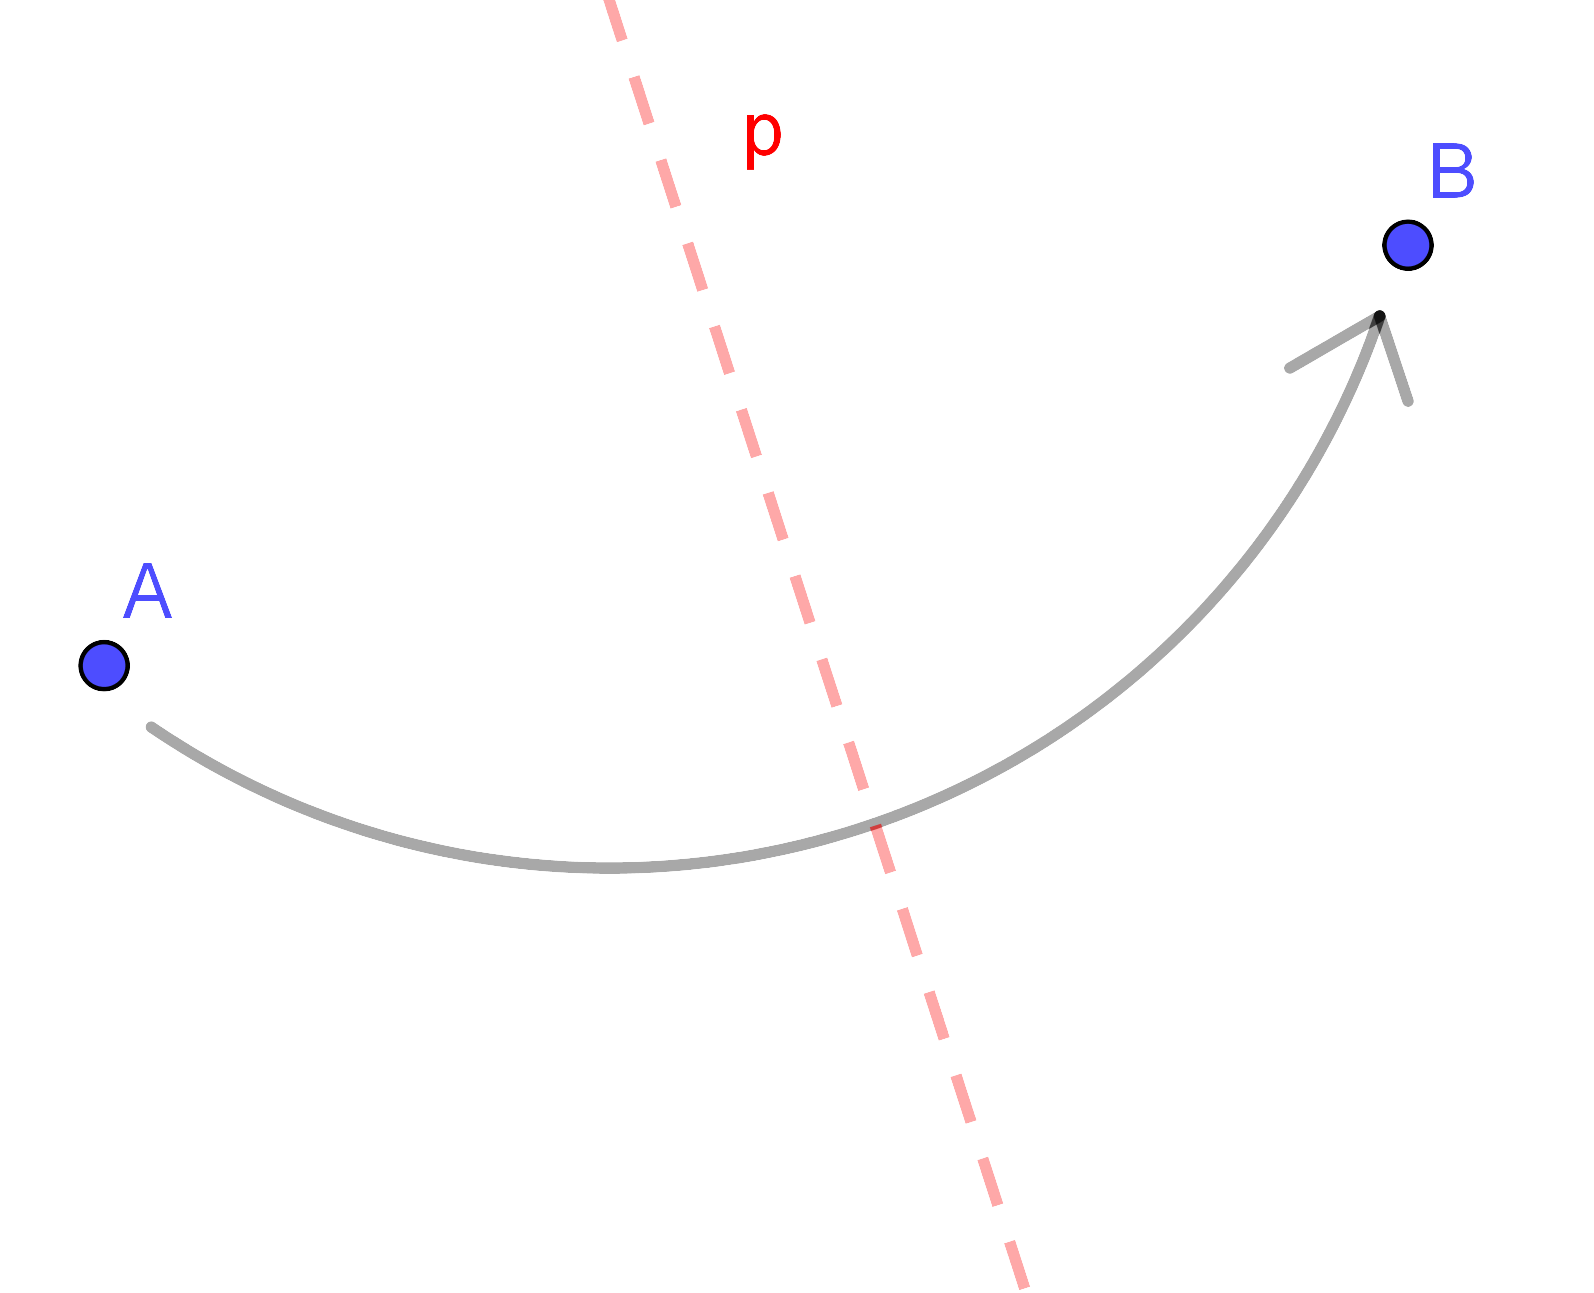
\includegraphics[width=0.35\textwidth]{images/origami_operacije/O3.png}
    \caption[Operacije~\ref{op:O1},~\ref{op:O2} in~\ref{op:O3}]{Operacije (od leve proti desni)~\ref{op:O1},~\ref{op:O2} in~\ref{op:O3}.}
    \label{fig:O1-O3}
\end{figure}

Nadalje opazimo, da nam operacija~\ref{op:O4} konstruira obe simetrali kota, ki ga določata premici in njuno presečišče, v primeru vzporednih premic pa dobimo tretjo vzporednico, ki leži na sredi med njima (slika~\ref{fig:O4}). Zato sta tu možna po dva ali, v posebnem primeru, en pregib.

\begin{figure}[h]
    \centering
    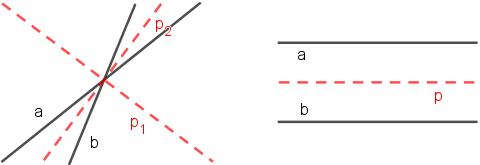
\includegraphics[width=0.5\textwidth]{images/origami_operacije/O4.png}
    \caption[Operacija~\ref{op:O4}]{Operacija~\ref{op:O4} v obeh možnih primerih.}
    \label{fig:O4}
\end{figure}

Operacija~\ref{op:O5} nam podaja konstrukcijo pravokotnice na premico skozi dano točko (slika~\ref{fig:O5}). Pri tem je vseeno, ali točka leži na premici ali ne. Pregib opravimo tako, da premico položimo samo nase in pazimo, da je točka $A$ v pregibu. Zaradi simetrije je pregib res pravokoten na premico in tako tudi en sam.

\begin{figure}[h]
    \centering
    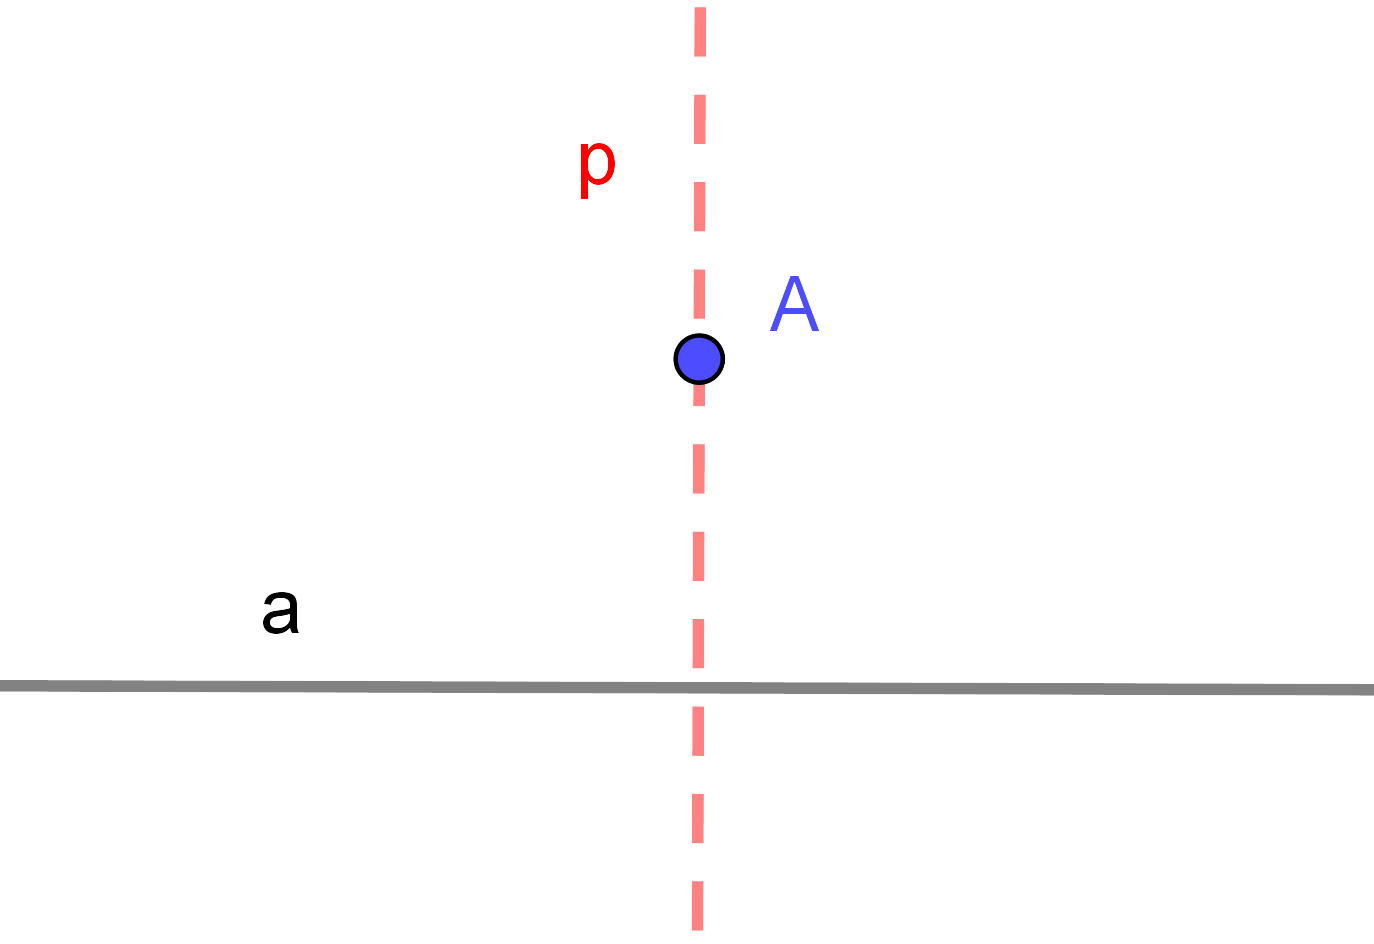
\includegraphics[width=0.35\textwidth]{images/origami_operacije/O5.png}
    \caption[Operacija~\ref{op:O5}]{Operacija~\ref{op:O5}.}
    \label{fig:O5}
\end{figure}

Operacija~\ref{op:O6} je še posebej zanimiva. Najprej si poglejmo njeno konstrukcijo. Vzemimo točki $A$ in $B$ ter premico $a$. Iščemo pregib skozi $B$, ki $A$ položi na premico $a$. Ker točka $B$ leži na pregibu, je enako oddaljena tako od točke $A$ kot tudi njene slike $A'$ na premici $a$, torej je $A'$ ravno presečišče premice $a$ in krožnice s središčem v $B$ ter polmerom $AB$. Pregib je simetrala daljice $AA'$, ki po konstrukciji poteka skozi točko $B$. Če velja $ d(A,B) > d(B,a) $, sta presečišči s premico $a$ dve (in s tem tudi dva možna pregiba, gl.\ sliko~\ref{fig:O6} levo), v primeru $ d(A,B) = d(B,a) $ je presečišče eno samo (in s tem en možen pregib, gl.\ sliko~\ref{fig:O6} na sredi) in je premica $a$ takrat tangentna na omenjeno krožnico, v zadnjem primeru, ko velja $ d(A,B) < d(B,a) $, pa presečišč ni (in s tem tudi pregiba, gl.\ sliko~\ref{fig:O6} desno).

\begin{figure}[h]
    \centering
    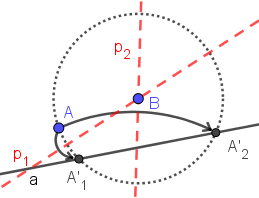
\includegraphics[width=0.55\textwidth]{images/origami_operacije/O6a.png}
    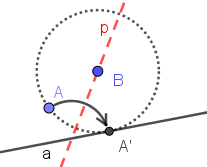
\includegraphics[width=0.2\textwidth]{images/origami_operacije/O6b.png}
    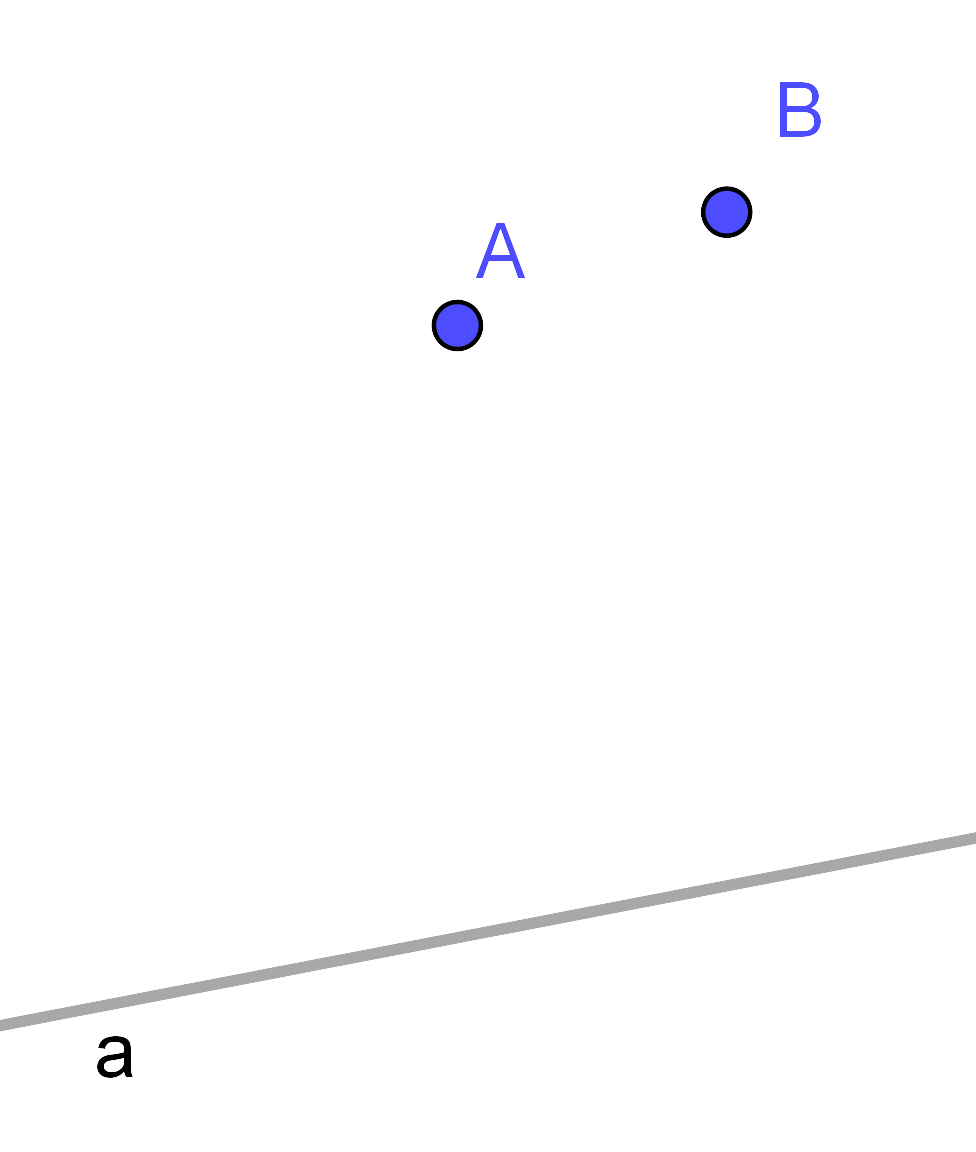
\includegraphics[width=0.2\textwidth]{images/origami_operacije/O6c.png}
    \caption[Operacija~\ref{op:O6}]{Operacija~\ref{op:O6} v vseh treh primerih.}
    \label{fig:O6}
\end{figure}

Zgodba operacije~\ref{op:O6} se tu še ne zaključi. Ker na pregibu ležijo vse točke, ki so enako oddaljene od točke $A$ in $A'$, to velja tudi za točko $P$, ki jo dobimo kot presečišče pregiba in pravokotnice na premico $a$ skozi $A'$ (slika~\ref{fig:O6_parabola}). Zanjo velja $ d(A,P) = d(P,a) $ in je enolično določena (v srednjem primeru na sliki~\ref{fig:O6} je to kar točka $B$). Torej točka $P$ leži na paraboli z goriščem $A$ in premico vodnico $a$. Bralec lahko sam premisli, da je $P$ edina točka na pregibu, ki je enako oddaljena od gorišča in premice vodnice. Pregib torej seka parabolo le v eni točki, kar pomeni, da je to \emph{tangenta na to parabolo}. V levem primeru na sliki~\ref{fig:O6} smo dobili dve tangenti.

\begin{figure}[h]
    \centering
    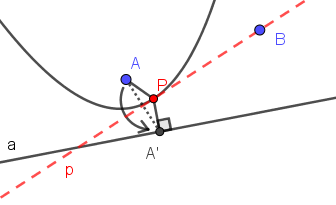
\includegraphics[width=0.6\textwidth]{images/origami_operacije/O6_parabola.png}
    \caption[Tangenta na parabolo]{Operacija~\ref{op:O6} kot konstrukcija tangente na parabolo z goriščem v $A$ in premico vodnico $a$.}
    \label{fig:O6_parabola}
\end{figure}

Poglejmo si naslednjo operacijo. Konstrukcijo~\ref{op:O7} začnemo z upogibom papirja, ki točko $A$ položi na premico $a$, potem pa točko premikamo po premici, dokler se tudi točka $B$ ne stakne s premico $b$. Takrat naredimo pregib. Na sliki~\ref{fig:O7} so prikazani trije pregibi, kar je tudi največje možno število pregibov za iste točke in premice. Več o številu pregibov sledi v razdelku~\ref{podpogl:kubicna_enacba}.

\begin{figure}[h]
    \centering
    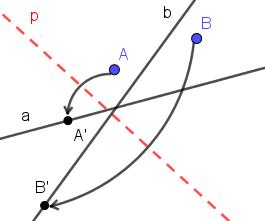
\includegraphics[width=0.35\textwidth]{images/origami_operacije/O7b.png}
    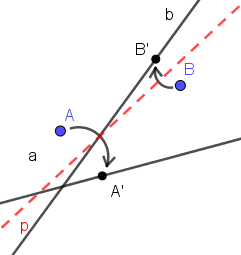
\includegraphics[width=0.3\textwidth]{images/origami_operacije/O7a.png}
    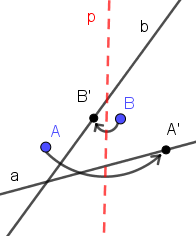
\includegraphics[width=0.3\textwidth]{images/origami_operacije/O7c.png}
    \caption[Operacija~\ref{op:O7}]{Operacija~\ref{op:O7} (primer treh pregibov za isti točki in premici).}
    \label{fig:O7}
\end{figure}

Kaj je geometrijski pomen te operacije? Če smo pri operaciji~\ref{op:O6} dobili tangento na parabolo, potem lahko takoj vidimo, da pri operaciji~\ref{op:O7} dobimo \emph{skupno tangento na dve paraboli} -- ena ima gorišče v točki $A$ in premico vodnico $a$, druga pa gorišče v točki $B$ ter premico vodnico $b$ (slika~\ref{fig:O7_paraboli}).

\begin{figure}[h]
    \centering
    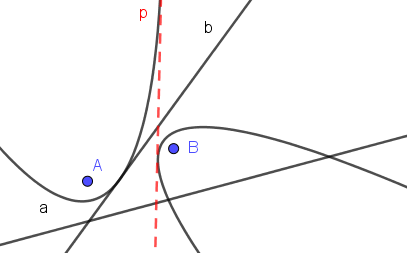
\includegraphics[width=0.7\textwidth]{images/origami_operacije/O7c_paraboli.png}
    \caption[Skupna tangenta na dve paraboli]{Operacija~\ref{op:O7} kot konstrukcija skupne tangente na dve paraboli.}
    \label{fig:O7_paraboli}
\end{figure}

\begin{opomba}
    O operaciji~\ref{op:O7} naj bi prva pisala italijanski matematičarki Margherita P.\ Beloch, po kateri operacijo imenujemo tudi \emph{Belochin pregib}.
\end{opomba}

Zadnja operacija~\ref{op:O8} zahteva nevzporedni premici, saj v nasprotnem primeru ne moremo konstruirati pregiba, ki bi bil pravokoten na obe premici in točko $A$ položil na premico $a$ (razen če le-ta že leži na njej). Premislimo geometrijsko konstrukcijo: ker mora biti pregib pravokoten na premico $b$, bo slika točke $A$ (označena z $A'$) ležala na vzporednici skozi točko $A$ k premici $b$. Prav tako mora točka $A'$ ležati na premici $a$, torej je slika ravno presečišče omenjene vzporednice in premice $a$. Iskan pregib je simetrala daljice $AA'$, ki je po konstrukciji pravokoten na premico $b$ (slika~\ref{fig:O8}).

\begin{figure}[h]
    \centering
    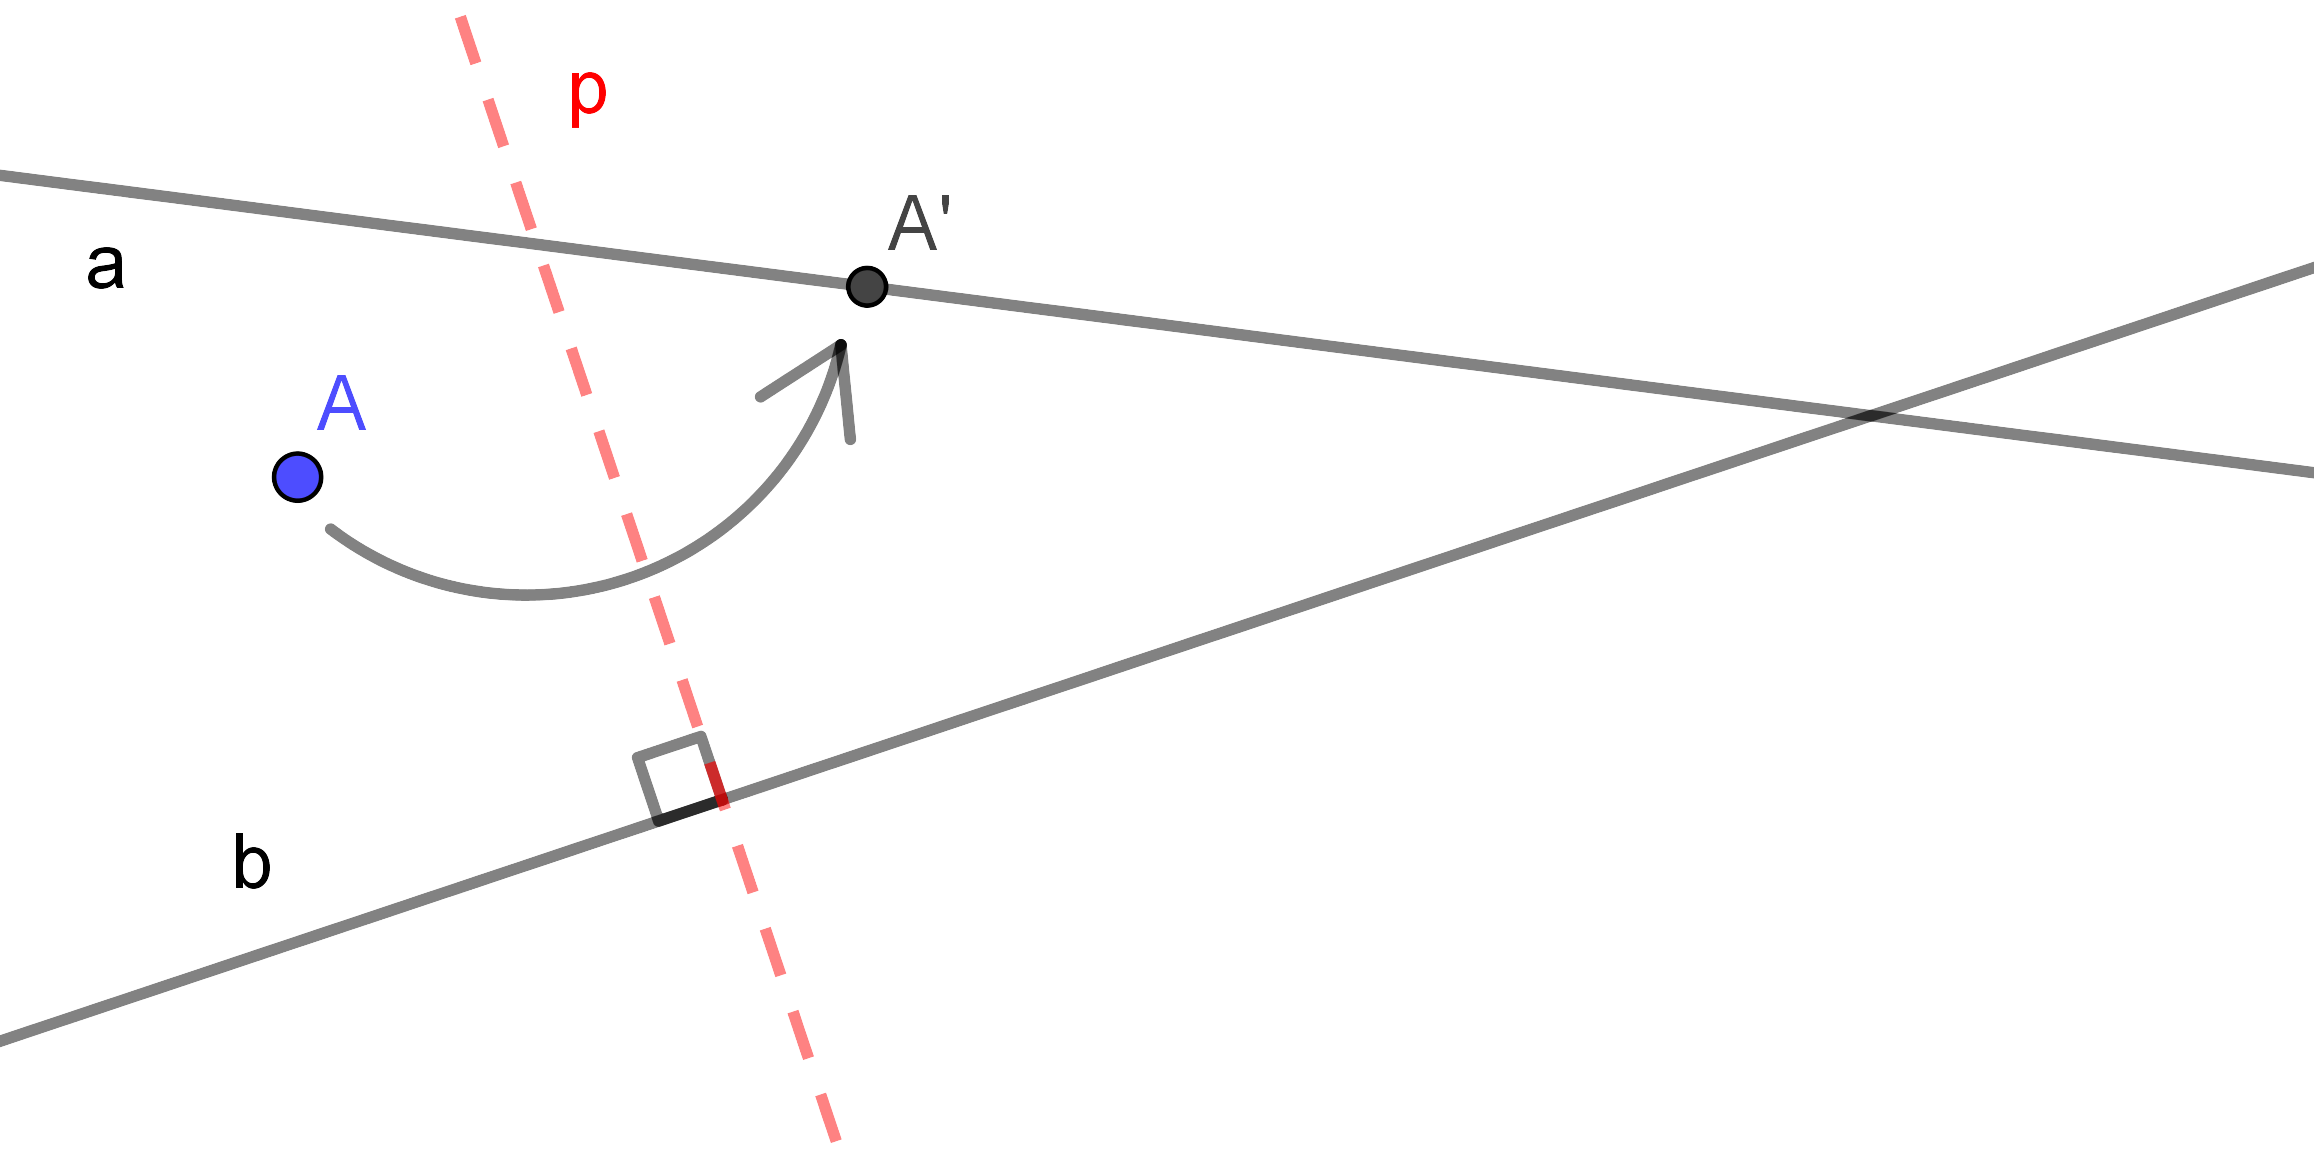
\includegraphics[width=0.6\textwidth]{images/origami_operacije/O8.png}
    \caption[Operacija~\ref{op:O8}]{Operacija~\ref{op:O8}.}
    \label{fig:O8}
\end{figure}

\opomba{Natančen bralec lahko opazi, da nam origami operacije ne podajajo konstrukcije slik točk, temveč samo pregibe, ki točke preslikajo na premice. Sliko točke konstruiramo šele po uporabi operacije~\ref{op:O5} -- skozi originalno točko naredimo pregib, pravokoten na prvi pregib (iz~\ref{op:O6}), in slika je potem presečišče pravokotnice in premice, na katero smo prepognili originalno točko.}

\subsubsection{Zadostne in potrebne origami operacije}
\label{podpogl:zadost_potr_op}

Omenili smo že, da je teh osem operacij zadostnih za katerokoli origami konstrukcijo.

\begin{izrek}
    \label{izr:op1do8}
    Če dovolimo le enkratne in ravne pregibe, so edine možne operacije prepogibanja operacije~\ref{op:O1}--\ref{op:O8}.
\end{izrek}

Ideja dokaza je, da za vsak možen prepogib, ki prekrije točko ali premico s točko ali premico (gl.\ seznam petih možnosti na začetku razdelka \ref{origami_konstrukcije}) pogledamo vse možnosti. Izkaže se, da res dobimo prepogibe iz operacij~\ref{op:O1}--\ref{op:O8}. Za natančen dokaz s slikovno ponazoritvijo gl.\ \cite[str.\ 24--26 (izrek 1.1)]{hull2020} \textcolor{red}{(Lahko tu dokažeš?)}.

Vendar ali so vse te operacije tudi potrebne ali lahko kakšno izpustimo? Operacija~\ref{op:O2} je očitno potrebna, saj nam določa nove točke. Če podrobneje opazujemo ostale konstrukcije, pa opazimo, da so vse posebni primeri operacije~\ref{op:O7} (t.\ j.\ konstrukcija pregiba, ki točko $A$ položi na premico $a$ in točko $B$ na premico $b$), ko premici $a$ in $b$ sovpadata ali ko ena ali obe izmed točk $A$ in $B$ ležita na premici:
\begin{itemize}
    \item Operacija~\ref{op:O1}: Naj točka $A$ leži na premici $a$, točka $B$ pa na premici $b$. Pregib skozi točki $A$ in $B$ točko $A$ ohrani na premici $a$ in točko $B$ na premici $b$.
    \item Operacija~\ref{op:O3}: Naj točka $A$ leži na premici $b$, točka $B$ pa na premici $a$. Pregib, ki položi točki drugo na drugo, točko $A$ položi na premico $a$ in hkrati točko $B$ na premico $b$ .
    \item Operacija~\ref{op:O4}: Naj točka $A$ leži na premici $b$, točka $B$ pa na premici $a$. Simetrala kota v presečišču premic (ali vmesna vzporednica, če sta premici $a$ in $b$ vzporedni), točko $A$ položi na premico $a$ in hkrati točko $B$ na premico $b$.
    \item Operacija~\ref{op:O5}: Naj točka $A$ leži na premici $a$, točka $B$ pa na premici $b$. Pregib skozi točko $A$ (ali $B$), ki je pravokoten na premico $b$ (ali $a$), točko $A$ ohrani na premici $a$ in točko $B$ na premici $b$.
    \item Operacija~\ref{op:O6}: Naj točka $B$ leži na premici $b$. Pregib skozi točko $B$, ki točko $A$ preslika na premico $a$ (če tak pregib obstaja), točko $B$ ohrani na premici $b$.
    \item Operacija~\ref{op:O8}: Naj točka $B$ leži na premici $b$. Pregib, ki točko $A$ položi na premico $a$ in je pravokoten na premico $b$, točko $B$ ohrani na premici $b$.
\end{itemize}

Ker lahko vse konstrukcije po izreku~\ref{izr:op1do8} opišemo z operacijami~\ref{op:O1}--\ref{op:O8}, smo s tem dokazali spodnji izrek:

\begin{izrek}
    \label{izr:dve_operaciji}
    Če imamo dani vsaj dve točki in dve nevzporedni (lahko tudi identični) premici, ki vsebujeta dane točke, potem lahko vse origami konstrukcije z enkratnimi in ravnimi pregibi opišemo s kombinacijo operacij~\ref{op:O2} in~\ref{op:O7}.
\end{izrek}

Vseeno bomo ohranili vseh osem aksiom operacij, saj bomo kakšen pregib lažje razložili preko ene od ostalih petih operacij kot pa opisovali, na kakšen način je to operacija~\ref{op:O7}.

\subsubsection{Zrcaljenje točke čez premico}
\label{zrcaljenje_origami}

Operacija~\ref{op:O3} nam poda simetralo daljice $AB$. Torej je točka $B$ zrcalna slika točke $A$ čez to premico. Kaj pa, če imamo za neko točko $A$ že dano premico $a$ in iščemo njeno zrcalno sliko? Naravna rešitev je, da naredimo pregib po premici in s svinčnikom označimo zrcalno sliko. A definicija~\ref{def:origami_konstruktibilnost} pravi, da lahko točke dobimo le kot presečišča pregibov, poleg tega pa je uporaba pisala dovoljena le za vidnejšo označbo že konstruiranih točk.

Zato moramo najti zaporedje pregibov, kjer na koncu kot presečišče nekih dveh premic dobimo želeno točko. Za dano premico $a$ in točki $A$, ki ne leži na tej premici (sicer je točka $A$ zrcalna slika sama sebi), lahko zrcalno sliko točke konstruiramo z naslednjimi koraki (prikazani na sliki~\ref{fig:zrcaljenje_cez_premico}, postopek vzet iz~\cite[str.\ 28]{hull2020}):
\begin{enumerate}
    \item Z operacijo~\ref{op:O5} prepognemo pravokotnico na premico $a$ skozi točko $A$.
    \item Z operacijo~\ref{op:O4} prepognemo simetralo kota, ki ga oklepata premica $a$ in pravokotnica iz prvega koraka.
    \item Z operacijo~\ref{op:O5} prepognemo pravokotnico na simetralo skozi točko $A$. Njeno presečišče s premico $a$ označimo z $B$.
    \item Z operacijo~\ref{op:O5} prepognemo pravokotnico na pregib iz tretjega koraka skozi točko $B$. Presečišče novega pregiba in pravokotnice iz prvega koraka označimo z $A'$.
\end{enumerate}

\begin{figure}[h]
    \centering
    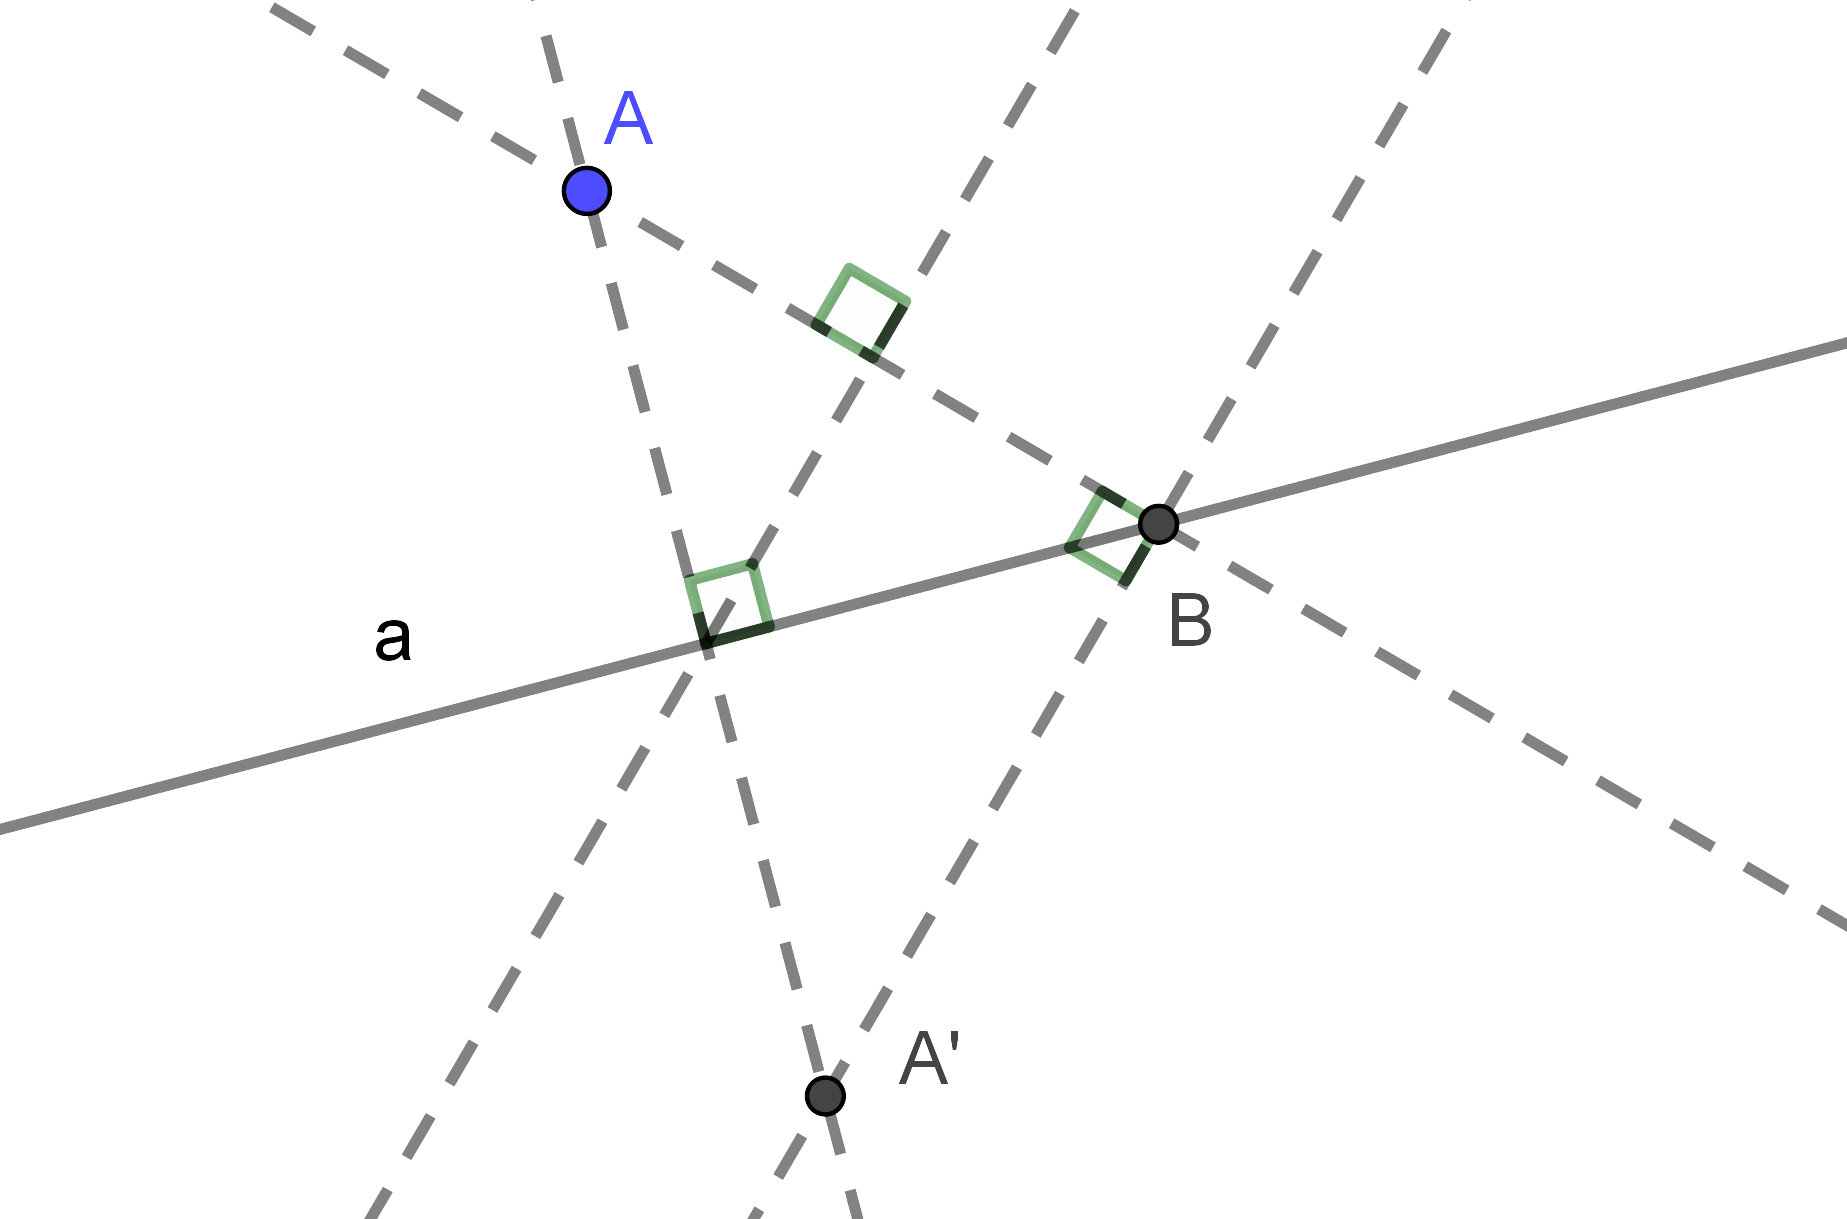
\includegraphics[width=0.5\textwidth]{images/zrcaljenje_tocke_cez_premico.png}
    \caption[Zrcaljenje čez premico]{Zrcaljenje točke $A$ čez premico $a$ s prepogibanjem papirja.}
    \label{fig:zrcaljenje_cez_premico}
\end{figure}

\begin{trditev}
    Točka $A'$ iz opisane konstrukcije je zrcalna slika točke $A$.
\end{trditev}

\begin{dokaz}
    Trikotnik, ki ga dobimo po 3.\ koraku, je pravokoten in enakokrak, saj je simetrala (pravega kota) iz 2.\ koraka pravokotna na njegovo osnovnico. Zato kot ob točki $A$ znaša $45^{\circ}$. Ker je trikotnik $\triangle A'BA$ pravokoten, je zato tudi enakokrak, torej premica $a$ razpolavlja daljico $AA'$, torej je $A'$ res zrcalna slika točke $A$.
\end{dokaz}

Ker lahko čez premico zrcalimo točke, lahko čeznjo zrcalimo tudi daljice oz.\ premice -- to storimo tako, da zrcalimo dve točki z daljice in naredimo pregib čez njuni sliki. Zrcaljenje pa nam omogoča še nekaj več, kar nam pove naslednja trditev.

% moja avtorska trditev in dokaz:)

\begin{trditev}
    \label{trd:prenasanje_razdalj}
    Z upoštevanjem pravil iz~\ref{origami_konstrukcije} in origami operacij lahko s prepogibanjem papirja prenašamo razdalje.
\end{trditev}

\begin{dokaz}
    V ravnini si izberimo poljubni točki $A$ in $B$, ki določata daljico z neko dolžino $r$. Naj bo $a$ poljubna premica in $A'$ poljubna točka na njej. Trditev pravi, da lahko z origami operacijami konstruiramo točko $B' \in a$, da je $d(A', B') =r$ (slika~\ref{fig:prenos_razdalje_konec}). Pri tem ni pomembno, na kateri strani točke $A'$ leži točka $B'$, saj jo lahko vedno zrcalimo čeznjo.

    \begin{figure}[h]
        \centering
        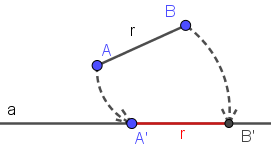
\includegraphics[width=0.5\textwidth]{images/zrcaljenje_konec.png}
        \caption[Prenašanje razdalj z origamijem]{Prenos dolžine daljice $AB$ na premico $a$ k izbrani točki $A'$.}
        \label{fig:prenos_razdalje_konec}
    \end{figure}
    
    Prenos razdalje razdelimo na dva koraka:
    \begin{enumerate}
        \item Če $A \neq A'$, daljico $AB$ zrcalimo čez tisto premico $p$, ki točko $A$ preslika v točko $A'$ (po~\ref{op:O3} je tak pregib oz.\ premica ena sama). Zrcalno sliko točke $B$ označimo z $B''$ (slika~\ref{fig:prenos_razdalje_koraki} levo). V posebnem primeru, ko daljica $AB$ leži na premici $a$, je to že konec konstrukcije. 
        \item Daljico $A'B''$ rotiramo okoli točke $A'$, da se točka $B''$ preslika na premico $a$. To storimo tako, da z operacijo~\ref{op:O4} konstruiramo simetralo kota med daljico $A'B''$ in premico $a$ in čeznjo zrcalimo točko $B''$ (slika~\ref{fig:prenos_razdalje_koraki} desno). S tem dobimo točko $B' \in a$, ki je po konstrukciji od točke $A'$ oddaljena za dolžino $r$.
    \end{enumerate}

    \begin{figure}[h]
        \centering
        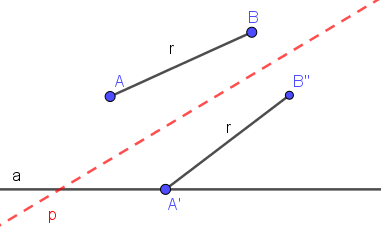
\includegraphics[width=0.45\textwidth]{images/zrcaljenje_korak1.png}
        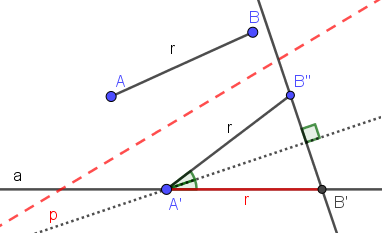
\includegraphics[width=0.45\textwidth]{images/zrcaljenje_korak2.png}
        \caption[Prenašanje razdalj z origamijem po korakih]{Zrcaljenje daljice $AB$ (levo) in rotacija daljice čez eno krajišče (desno).}
        \label{fig:prenos_razdalje_koraki}
    \end{figure}

    S tem smo razdaljo $r$ prenesli na poljubno mesto v ravnini.
\end{dokaz}

Tako lahko s prepogibanjem papirja zrcalimo točke (in premice), prenašamo razdalje pa tudi -- po 2.\ koraku iz zgornjega dokaza -- rotiramo točke (in premice). To novo znanje bomo uporabili v razdelku~\ref{origami_konstruktibilnost}, od sedaj naprej pa bomo pri konstrukcijah, ki vključujejo zrcaljenje točk, zaradi preglednosti izpustili potrebne pregibe in zrcaljene točke označili kar s svinčnikom skozi papir.

\subsection{Zakaj origami konstrukcije nadvladajo evklidske}
\label{podpogl:nadvlada_origamija}

Prišli smo do ključnega dela poglavja -- reševanje vprašanja, zakaj se nam z origami konstrukcijami sploh splača ukvarjati.

Tako z evklidskim orodjem kot s prepogibanjem papirja lahko konstruiramo premice in točke ter prenašamo razdalje. Le evklidskim orodjem lahko konstruiramo tudi krožne loke, ker pa znamo rotirati točke okoli druge točke, lahko tudi s prepogibanjem papirja konstruiramo katerokoli točko na krožnici z danim središčem in polmerom. Tako lahko vse evklidske konstrukcije opravimo tudi z origamijem (za natančnejši dokaz gl.\ \cite{robert1995}).

Bralec je ob zgornjih opisih posamezne operacije povabljen, da premisli, kako je mogoče operacije~\ref{op:O1}, \ref{op:O3}, \ref{op:O4}, \ref{op:O5}, \ref{op:O6} in \ref{op:O8} opraviti tudi z evklidskim orodjem (operacija~\ref{op:O2} le določa nove točke, zato tu o konstrukciji ne moremo govoriti). Do tu nam torej origami konstrukcije niso dale ničesar novega.

Ključna je sedma operacija. Izkaže se namreč, da operacije~\ref{op:O7} oz.\ Belochinega pregiba ne moremo opraviti z evklidskim orodjem. Kako lahko to dokažemo? V razdelku~\ref{podpogl:trisekcija} bomo spoznali več origami postopkov, ki nam poljuben kot razdelijo na tri skladne dele, pri tem pa uporabimo pregib iz operacije~\ref{op:O7}. Ker \emph{trisekcija kota z evklidskim orodjem ni mogoča} (dokaz v~\cite[str.\ 77--78]{jerman1998}), posledično tudi konstrukcija operacije~\ref{op:O7} s tem orodjem ne obstaja. Prav tako bomo v poglavju~\ref{pogl:enacbe} videli več načinov uporabe operacije~\ref{op:O7} za reševanje kubične enačbe, za katero prav tako vemo, da je v splošnem z evklidskim orodjem ne moremo rešiti.

Sedaj vemo, da je množica evklidskih konstrukcij \emph{prava} podmnožica origami konstrukcij. V naslednjem razdelku si bomo pogledali, kako lahko evklidske in origami konstrukcije prevedemo v jezik algebre in tudi na algebrski način pokažemo premoč origamija nad evklidskim orodjem. Raziskovali bomo, katere dolžine (in s tem katera števila) lahko z obema orodjema konstruiramo. Tak pogled je imel že Evklid, ki je na števila gledal kot končni rezultat niza konstrukcij z evklidskim orodjem pri dani daljici enotske dolžine~\cite[str. 164]{michael2005}.

\subsubsection{Algebrski pogled na evklidske konstrukcije}
\label{podpogl:evkl_konstruktibilnost}

\begin{definicija}
    Na listu papirja, ki nam služi kot model ravnine $\C$, imejmo dano izhodišče $O$ in število $1$ na realni osi. Če lahko z neoznačenim ravnilom in šestilom s končnim številom potez konstruiramo kompleksno število $\alpha$, rečemo, da je $\alpha$ \emph{evklidsko-konstruktibilno} število.
\end{definicija}

\begin{opomba}
    Ker lahko z neoznačenim ravnilom in šestilom konstruiramo le daljice, poltrake in premice skozi dani točki (postulata~\ref{post:P1} in~\ref{post:P2}) ter krožnice z danim središčem in polmerom (postulat~\ref{post:P3}), lahko nove točko konstruiramo le kot presečišče dveh premic, dveh krožnic ali premice in krožnice.
\end{opomba}

Jerman bralca v~\cite{jerman1998} (zelo nazorna je tudi izpeljava v~\cite[str.165--170]{michael2005}) na zelo strukturiran in nazoren način popelje čez dokaz, da lahko z evklidskim orodjem na realni osi konstruiramo natanko vsa racionalna števila, njihove vsote, razlike, zmnožke, količnike, kvadratne korene ter linearne kombinacije vsega naštetega. To je množica
$$
    \Q(r) = \{ a + b \sqrt{r}; a, b, r \in \Q; r > 0 \text{ in } \sqrt{r} \notin \Q \},
$$
ki je komutativen obseg oz.\ polje in hkrati tudi dvorazsežni vektorski prostor nad obsegom $\Q$ z bazo $ \{1, \sqrt{r} \} $.

Da pokažemo, da so to vsa možna realna evklidsko-konstruktibilna števila, je potrebna obravnava vseh možnih enačb, ki jih dobimo pri iskanju presečišč dveh krožnic, dveh premic ter krožnice in premice, potem pa je potrebno še dokazati, da nam vse nadaljne rabe konstruiranih presečišč res podajo najmanjšo razširitev polja racionalnih števil, ki je zaprta za operacijo kvadratnega korenjenja. Jerman s tem dokaže naslednji izrek.

\begin{izrek}
    \label{izr:evkl_konstr}
    Število $r \in \R$ se da konstruirati le s pomočjo ravnila in šestila natanko tedaj, ko je $r$ algebraičen nad $\Q$ in je razsežnost obsega $\Q(r)$, kot vektorskega prostora nad obsegom $\Q$, enaka $2^n$ za nek $n \in \N_0$.
\end{izrek}

\begin{opomba}
    \label{op:razseznost_obsega_evkl}
    Razsežnosti obsega $\Q(r)$ pravimo tudi \emph{stopnja razširitve obsega $\Q$}. Izkaže se, da je enaka stopnji minimalnega polinoma števila $r$ nad $\Q$~\cite[str.\ 77]{jerman1998}.
\end{opomba}

Izreku takoj sledita dokaza, da trisekcija kota v splošnem ter konstrukcija števila $ \sqrt[3]{2} $ z evklidskim orodjem nista mogoči~\cite[str.\ 77--78]{jerman1998}.

Iz izreka sledi tudi, da lahko vsa realna evklidsko-konstruktibilna števila analitično zapišemo kot rešitve kvadratne enačbe z racionalnimi koeficienti. O reševanju enačb se bomo natančneje ukvarjali v poglavju~\ref{pogl:enacbe}.

Ker med kompleksno in evklidsko ravnino obstaja bijekcija, lahko tako konstruiramo poljubno število $\alpha = x + y i$, kjer sta $x \in \Q(r)$ in $y \in \Q(s)$ za neka $r, s \in \Q^+; \sqrt{r}, \sqrt{s} \notin \Q$. S tem lahko zapišemo tudi kompleksne rešitve kvadratne enačbe. Torej lahko z evklidskim orodjem konstruiramo rešitve poljubne kvadratne enačbe.

\subsubsection{Origami števila}
\label{origami_konstruktibilnost}

Poiščimo še množico števil, ki jih lahko konstruiramo z origamijem. Definiramo jih na enak način kot \emph{evklidsko-konstruktibilna} števila.

\begin{definicija}
    \label{def:origami_stevilo}
    Na listu papirja, ki nam služi kot model ravnine $\C$, imejmo dano izhodišče $O$ in število $1$ na realni osi. Premice predstavljajo pregibi papirja, nove točke pa njihova presečišča. Če lahko s končnim številom enkratnih ravnih prepogibov in upoštevanjem operacij~\ref{op:O1}--~\ref{op:O8} konstruiramo kompleksno število $\alpha$, rečemo, da je $\alpha$ \emph{origami število}. Množico origami števil označimo z $\mathcal{O}$.
\end{definicija}

\begin{opomba}
    Po izreku~\ref{izr:op1do8} operacije~\ref{op:O1}--~\ref{op:O8} zajamejo vse možne pregibe, zato so origami števila dobro definirana.
\end{opomba}

\begin{definicija}
    Če lahko v evklidski ravnini z origamijem po zgornjih pravili konstruiramo točko $A$, pravimo, da je $A$ \emph{origami-konstruktibilna točka}. Če lahko z origamijem konstruiramo premico $p$, pravimo, da je premica $p$ \emph{origami-konstrukcibilna premica}.
\end{definicija}

Preko sledečih izrekov in trditev bomo še na algebrski način pokazali, da je množica števil, ki jih lahko konstruiramo z evklidskim orodjem, prava podmnožica množice origami števil.

\begin{trditev}
    \label{trd:zaprt_koord}
    Naj bo $\alpha = a + bi \in \C$, kjer $a, b \in \R$. Potem je $\alpha \in \mathcal{O}$, če in samo če $a, b \in \mathcal{O}$.
\end{trditev}
\begin{dokaz}
    Ker sta $a$ in $b$ pravokotni projekciji števila $\alpha$ na realno in imaginarno os (operacija~\ref{op:O5}), je trditev očitna.
\end{dokaz}

\begin{izrek}
    \label{izr:podpolje}
    Množica $\mathcal{O}$ je podpolje polja $\C$.
\end{izrek}

\begin{dokaz}
    Za dokaz izreka moramo pokazati, da je $1 \in \mathcal{O}$ (kar velja že po definiciji), da za poljubna $\alpha, \beta \in \mathcal{O}$ velja $\alpha - \beta, \alpha\beta \in \mathcal{O}$ in da je $1/\alpha \in \mathcal{O}$ za vsak $\alpha \in \mathcal{O} \backslash \{0\}$. Spomnimo se, da lahko kompleksna števila ponazorimo z vektorji in zato lahko računske operacije grafično izvajamo kar preko njih.

    Vzemimo poljubna $\alpha, \beta \in \mathcal{O}$. Ker število $-\beta$ dobimo po zaporednem zrcaljenju čez obe osi, velja $-\beta \in \mathcal{O}$. Ker je odštevanje v resnici seštevanje nasprotnega elementa, je za dokaz $\alpha - \beta \in \mathcal{O}$ dovolj pokazati, da je množica $\mathcal{O}$ zaprta za seštevanje.

    Če $\alpha, \beta$ in $O$ ležijo na isti premici, ni veliko za dokazovati, temveč samo prenesemo razdaljo na primerno mesto na premici. Predpostavimo sedaj, da $\alpha, \beta$ in $O$ ne ležijo na isti premici in s paralelogramskim pravilom konstrirajmo število $\alpha + \beta$ (slika~\ref{fig:sestevanje}). Štirikrat uporabimo operacijo~\ref{op:O5}: preko pravokotnice $(1)$ na vektor $\overrightarrow{O\beta}$ skozi $\alpha$ konstruiramo vzporednico $(2)$ k taistemu vektorju skozi $\alpha$ in na enak način preko pravokotnice $(3)$ konstruiramo vzporednico $(4)$ k vektorju $\overrightarrow{O\alpha}$ skozi $\beta$. V presečišču vzporednic dobimo $\alpha + \beta$.

    \begin{figure}[h]
        \centering
        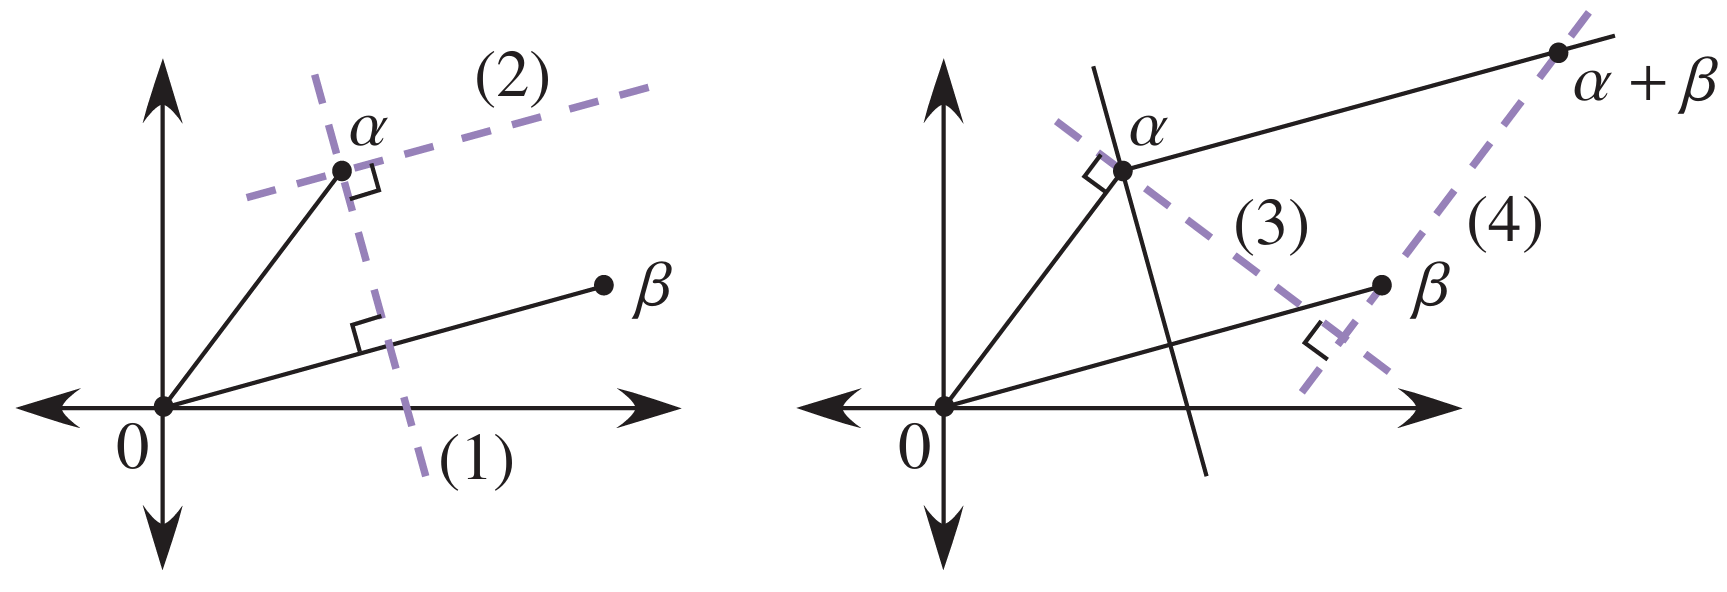
\includegraphics[width=0.7\textwidth]{images/algebra/sestevanje.png}
        \caption[Seštevanje origami števil]{Konstrukcija $\alpha + \beta$.}
        \label{fig:sestevanje}
    \end{figure}

    Za dokaz preostalih dveh zahtev najprej dokažimo, da za neničelna $a, b \in \mathcal{O} \cap \R$ velja $ab, 1/a \in \mathcal{O}$, potem pa s pomočjo trditve~\ref{trd:zaprt_koord} to dokažemo še za poljubna $\alpha, \beta \in \mathcal{O}$.

    Naj bosta $a, b \in \mathcal{O} \cap \R$ poljubna in neničelna (če je katerikoli od njiju enak $0$, je produkt ničeln in že po definiciji origami število). Ker sta $a$ in $b$ origami števili, ju lahko konstruiramo. Naj $b$ leži na realni osi, $ai$ pa na imaginarni (slika~\ref{fig:mnozenje_deljenje} levo). Z dvakratno uporabo operacije~\ref{op:O5} konstruiramo origami število $1 + ai$ (točka $B$). Konstruiramo pregib skozi $O$ in $B$ (premica z naklonom $a$) ter v presečišču s pravokotnico skozi $b$ dobimo število $b + abi$ (točka $C$). Pravokotnica skozi $C$ na imaginarno os na njej konstruira origami število $ab$.

    \begin{figure}[h]
        \centering
        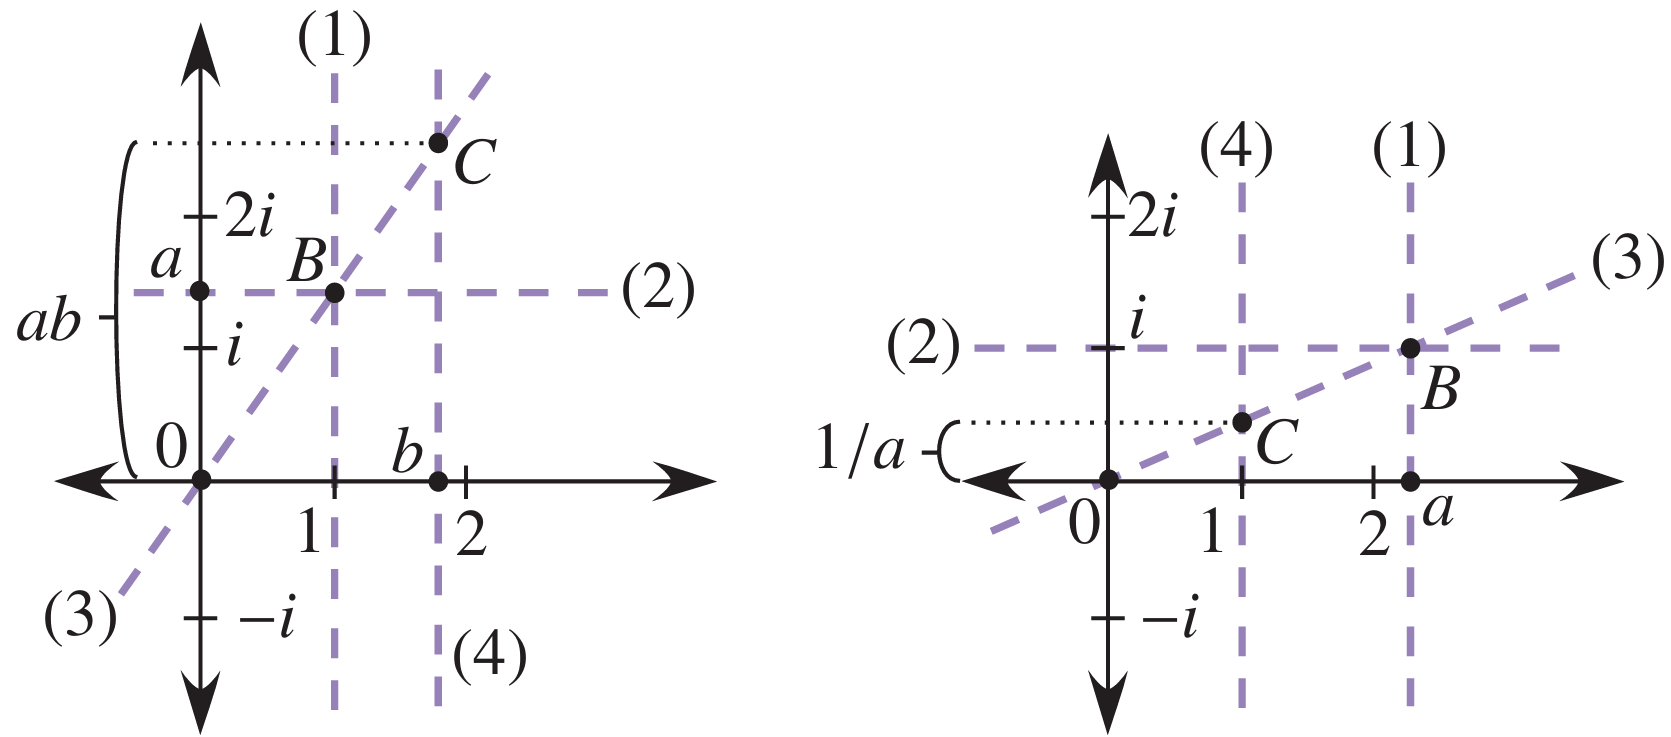
\includegraphics[width=0.7\textwidth]{images/algebra/mnozenje_deljenje.png}
        \caption[Množenje in obratna vrednost realnih origami števil]{Konstrukcija $ab$ in $1/a$ za neničelna $a, b \in \mathcal{O} \cap \R$.}
        \label{fig:mnozenje_deljenje}
    \end{figure}

    Podobno konstruiramo še število $1/a$. Na realni osi konstruiramo število $a$ (slika~\ref{fig:mnozenje_deljenje} desno), s pomočjo~\ref{op:O5} pa še število $a + i$ (točka $B$). Pregib skozi $O$ in $B$ ima naklon ravno $1/a$. V presečišču tega pregiba s pravokotnico na realno os v točki $!$ dobimo število $1 + (1/a) i$ (točka $C$). Tako nam pravokotnica na imaginarno os skozi točko $C$ konstruira origami število $1/a$.

    Vzemimo sedaj poljubna $\alpha, \beta \in \mathcal{O}$. Če je $\alpha = a + bi, \beta = c + di$, potem po trditvi~\ref{trd:zaprt_koord} velja $a, b, c, d \in \mathcal{O}$. Število $\alpha \beta = (ac - bd) + (ad + bc)i$ ima v svojem realnem in imaginarnem delu njihove vsote, razlike in produkti, za katere že vemo, da so v $\mathcal{O}$. Torej je $\alpha, \beta \in \mathcal{O}$.

    Za neničeln $\alpha = a + bi \in \mathcal{O}$ je $1/\alpha = a/(a^2+b^2) + (-b)/(a^2+b^2)i$. Ker sta po trditvi~\ref{trd:zaprt_koord} $a, b \in \mathcal{O}$, sta zopet realni in imaginarni del tega števila origami števili, torej $1/\alpha \in \mathcal{O}$.
\end{dokaz}

\begin{trditev}
    \label{trd:zaprtost_koren}
    Naj bo $\alpha \in \mathcal{O}$. Potem $\sqrt{\alpha}, \sqrt[3]{\alpha} \in \mathcal{O}$.
\end{trditev}

\begin{dokaz}
    Naj bo $\alpha = r e^{i \theta}$ za neka $r \in \R \backslash \{0\}$ (v ničelnem primeru ni kaj dokazovati) in $\theta$ poljuben kot. Torej imamo za kvadratni in kubični koren števila $\alpha$ skupno pet rešitev:
    \begin{itemize}
        \item $\sqrt{\alpha} = \pm \sqrt{r}e^{i \frac{\theta}{2}}$ in
        \item $\sqrt[3]{\alpha}_1 = \sqrt[3]{r}e^{i \frac{\theta}{3}}, \sqrt[3]{\alpha}_2 = \sqrt[3]{r}e^{i \left(\frac{\theta}{3} + \frac{2\pi}{3}\right)}, \sqrt[3]{\alpha}_3 = \sqrt[3]{r}e^{i \left(\frac{\theta}{3} + \frac{4\pi}{3}\right)}$.
    \end{itemize}
    Torej moramo dokazati, da $\sqrt{r}, \sqrt[3]{r} \in \mathcal{O}$, da znamo razpolavljati in tretjiniti kote ter rotirati origami število za kot $60^\circ$ okoli izhodišča $O$. Potem bomo po izreku~\ref{izr:podpolje} lahko konstruirali zgornjih pet števil in tako dokazali to trditev.

    Najprej se še prepričajmo, da $r \in \mathcal{O}$. Ker je to ravno razdalja števila $\alpha$ do izhodišča, jo lahko prenesemo na realno os in tako konstruiramo realno število $r$, torej je res $r \in \mathcal{O}$.
    
    V razdelku~\ref{pogl:enacbe} bomo pogledali, kako z origamijem rešujemo splošne kvadratne in kubične enačbe, torej bomo znali konstruirati tudi rešitve enačb $x^2 - r = 0$ in $x^3 - r = 0$. Konkretne konstrukcije števil $\sqrt{r}$ in $\sqrt[3]{r}$ opisane tudi v poglavju~\ref{pogl:prepog_kvadrata}. Z operacijo~\ref{op:O4} znamo razpoloviti kot, postopek tretjinjenja kota pa je, kot že omenjeno, opisan v razdelku~\ref{podpogl:trisekcija}. Ostane nam samo še rotacija točke za kot $60^\circ$ okoli izhodišča. Na sliki~\ref{fig:kot60_rotacija} je prikaz enostavne konstrukcije -- najprej prepognemo simetralo $p_1$ daljice $OA$ in konstruiramo pregib $p_2$ skozi $O$, ki točko $A$ preslika v točko $A'$ na simetrali $p_1$. Trikotnik $\triangle OAA'$ je enakostraničen. 
    \begin{figure}[h]
        \centering
        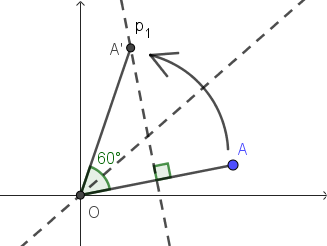
\includegraphics[width=0.5\textwidth]{images/algebra/kot60.png}
        \caption[Rotacija točke okoli izhodišča]{Rotacija točke za kot $60^\circ$ okoli izhodišča.}
        \label{fig:kot60_rotacija}
    \end{figure}
\end{dokaz}

Množica origami števil $\mathcal{O}$ je tako zaprta za seštevanje, odštevanje, množenje, deljenje ter za kvadratno in kubično korenjenje. Ker so cela števila očitno origami števila (po definiciji imamo dano enoto, ki jo znamo prenašati po realni osi), so zaradi zaprtosti za deljenje origami števila tudi vsa racionalna števila. Zato za vsak $r \in \Q^+, \sqrt{r} \notin \Q$ in vsaka $a, b \in \Q$ velja $a + b\sqrt{r} \in \mathcal{O}$, torej za vsak tak $r$ velja
$$ \Q(r) \subseteq \mathcal{O}. $$
S tem je dokazana naslednja trditev.

\begin{trditev}
    Vsa evklidsko-konstruktibilna števila so origami števila.
\end{trditev}

Da so evklidsko-konstruktibilna števila \emph{prava} podmnožica origami števil, je potrebno najti samo en $r \in \mathcal{O} \cap \Q^+, \sqrt{r} \notin \Q$, za katerega velja $\sqrt[3]{r} \notin \Q(r)$. Bralec je povabljen k enostavnemu dokazu, da že za $r = 2$ ne obstajata $a, b \in \Q$, da bi veljalo $\sqrt[3]{2} = a + b\sqrt{2}$ -- če začnemo reševati to enačbo za $a$ in $b$, se hitro izkaže, da nima niti realnih rešitev.

\begin{izrek}
    Množica evklidsko-konstruktibilnih števil je prava podmnožica množice origami števil, t.\ j.
    $$ \bigcup_{r \in \Q^+, \sqrt{r} \notin \Q} \Q(r) \subset \mathcal{O} $$
\end{izrek}

Tako smo še na algebraičen način dokazali prevlado origamija nad evklidskim orodjem.

\textcolor{red}{(a potem so origami števila enaka množici $\{ a + b \sqrt{r} + c \sqrt[3]{q} \}$ za poljubne $a, b, c, r, q \in \Q$? Je kakšna oznaka?)}

\textcolor{red}{A vključimo še ta izrek, da bo podobno kot~\ref{izr:evkl_konstr}? Lahko gledajo Alperin~\cite{alperin2000}}

\begin{izrek}
    \label{izr:origami_konstr}
    Število $r \in \R$ se da konstruirati z origamijem natanko tedaj, ko je $r$ algebraičen nad $\Q$ in je razsežnost obsega $\Q(r)$, kot vektorskega prostora nad obsegom $\Q$, enaka $2^n 3^m$ za neka $n, m \in \N_0$.
\end{izrek}
